% !TeX root = Trafficsimulation_Documentation.tex

\chapter{Implementierung}
\label{Implementierung}

In diesem Kapitel werden die Implementierungen der einzelnen Komponenten sowie deren Schnittstellen zu anderen Komponenten dokumentiert.

\thispagestyle{standard}
\pagestyle{standard}

\section{Erstellung der Welt}
\label{Erstellung der Welt}

\section{Fahrzeugsteuerung}
\label{Fahrzeugsteuerung}
% Inklusive Abbiegen, Weg folgen, Spawn

\section{Erkennen und Reagieren auf Ampeln}
\label{Erkennen und Reagieren auf Ampeln}

\section{Fahrzeug Kollisionserkennung}
\label{Fahrzeug Kollisionserkennung}

\section{Ampelsteuerung}
\label{Ampelsteuerung}

Die Ampelsteuerung wurde als eigene Applikation entwickelt. Die Ampelsteuerung kann grundsätzlich unabhängig von der Unity-Spielwelt laufen, auch die Ampeln schalten dementsprechend autonom, auch wenn die Simulation schon beendet sein sollte.

... evtl. mike wos


Die Ampelsteuerung ist auch mit Mono lauffähig. Mono ist eine C_#-Implementierung für unixoide Betriebssysteme. So läuft die Ampelsteuerung auch mit Linux. Auch eine Kompilierung ist möglich, mit \texttt{xbuild solution.sln} wird eine ausführbare Datei erzeugt, die sowohl mit Linux als auch Windows lauffähig ist.

In Abbildung \ref{img:ampel} ist die Ausgabe der Ampelsteuerung zu sehen. Da die Ampelsteuerung gut funktionierte, wurde in die Ausgabe weniger Zeit investiert, sodass hier nur die aufrufende IP ausgegeben wird.

\begin{figure}[H]
\begin{center}
	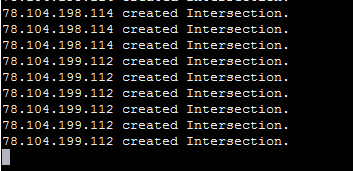
\includegraphics[width=0.9\textwidth]{BilderAllgemein/ampelserver.png}
\end{center}

	\caption{Ausgabe Ampelserver}

	\label{img:ampel}
\end{figure}



\section{Erstellen und Löschen von Hindernisse}

Um im Environment Hindernisse zur Laufzeit zu Erstellen, muss dem Terrain-GameObject ein Skript (Obstacles.cs) hinzugefügt werden. In diesem Skript findet die Abarbeitung des Inputs des Users statt.

Wie bereits in \ref{Hindernisse} erläutert wird zum Start der Verkehrssimulation das Hindernis geladen. Dies erfolgt über den "Load" Befehl.

\begin{lstlisting}[caption={Laden des Hindernisses},label={lst:Hinderniss_laden}]
private GameObject prefabLog;
void Start()
{
	prefabLog = Resources.Load("Rock", typeof(GameObject)) as GameObject;
}
\end{lstlisting}

Der in \ref{Hindernisse} beschrieben soll ein Button gedrückt gehalten werden um Hindernisse spawnen zu können. Dieser wird über einen KeyCode definiert. Im Skript wird nun in jedem Update Aufruf darauf gewartet, ob der definierte Button gedrückt und ein "MouseDown" Event vorkommt. Mit diesem Event kann die Position der Maus auf dem Bildschirm herausgefunden werden, jedoch stimmen diese nicht mit den Welt-Koordinaten überein. Deshalb muss hier eine Umwandlung durchgeführt werden, welche mit Hilfe eines Raycasts gelöst wurde. Durch das Instanzieren wird das neu erstellte Hindernis in der Welt platziert.

\begin{lstlisting}[caption={Erstellen des Hindernisses},label={lst:Hinderniss_erstellen}]
private KeyCode shiftLeft = KeyCode.LeftShift;
if(Input.GetMouseButtonDown(0) && Input.GetKey(shiftLeft)) //Left mouse button clicked
{
	Vector3 mousePosition = Input.mousePosition;
	var ray = Camera.main.ScreenPointToRay(mousePosition);
	RaycastHit hit;
	if(Physics.Raycast(ray, out hit, 1000f))
	{
		Vector3 position = hit.point;			Vector3 yOffset = new Vector3(0, 1.5f, 0);
		position += yOffset;			
		GameObject prefabInstance = Instantiate(prefabLog, position, new Quaternion()) as GameObject;
	}
}
\end{lstlisting}

Zum Löschen eines Hindernisses muss die rechte Maustaste in Kombination mit dem vorher definierten Button verwendet werden. Mittels "Destroy" wird anschließend das erkannte GameObject wieder von der Welt gelöscht.

\begin{lstlisting}[caption={Zerstören des Hindernisses},label={lst:Hinderniss_zerstören}]
if(Input.GetMouseButtonDown(1) && Input.GetKey(shiftLeft)) //Right mouse button clicked
{
	Vector3 mousePosition = Input.mousePosition;
	var ray = Camera.main.ScreenPointToRay(mousePosition);
	RaycastHit hit;
	if(Physics.Raycast(ray, out hit, 1000f))
	{
		Vector3 position = hit.point;
		GameObject collidedObject = hit.collider.gameObject;
		if(collidedObject.name.Equals("Rock(Clone)"))
		{
			Destroy(collidedObject);
		}
	}
}
\end{lstlisting}

\begin{figure}[H]
\begin{center}
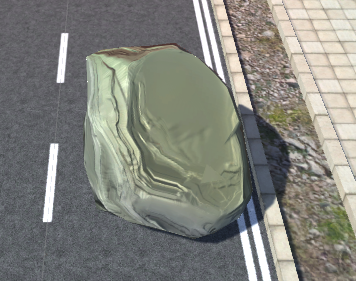
\includegraphics[width=0.5\textwidth]{BilderAllgemein/rock.PNG}
\end{center}
	\caption{Hindernis}
	\label{img:hindernis}
\end{figure}

\section{Aus- und Einfahren von Fahrzeugen anderer Gruppen}
\label{Aus- und Einfahren von Fahrzeugen anderer Gruppen}

Mit dem Plugin `Unity3D.Amqp` (\url{https://github.com/CymaticLabs/Unity3D.Amqp}) für Unity ist es möglich einen RabbitMQ-Server direkt in Unity einzubinden.

Die Konfiguration der Serverdaten werden dabei direkt in den Menüeinstellungen von Unity vorgenommen. Die verwendete Konfiguration ist in Abbildung \ref{img:rabbit} zu sehen.

\begin{figure}[H]
\begin{center}
	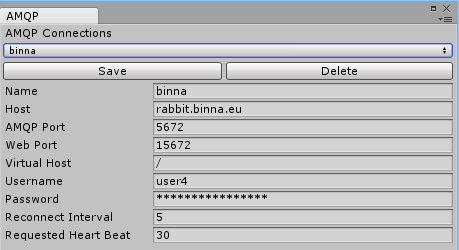
\includegraphics[width=0.9\textwidth]{BilderAllgemein/rabbitconfig.png}
\end{center}

	\caption{Einstellungen RabbitMQ}

	\label{img:rabbit}
\end{figure}

Jede Gruppe bekam einen eigenen Benutzer samt Passwort. Damit man Nachrichten empfangen kann, muss man sich auf eine `Queue` subscriben.

Das Plugin stellt anschließend Methoden zur Verfügung. Eine solche Methode ist \texttt{OnMessageReceived()}. Damit lässt sich eine eingehende Nachricht an ein Objekt in der Spielwelt weitergeben. Das Objekt kann daraufhin reagieren, beispielsweise ein Auto erzeugen.

\begin{figure}[H]
\begin{center}
	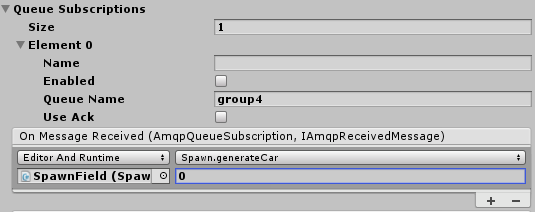
\includegraphics[width=0.9\textwidth]{BilderAllgemein/rabbitqueue.png}
\end{center}

	\caption{RabbitMQ Queue}

	\label{img:rabbitq}
\end{figure}

In Abbildung \ref{img:rabbitq} sieht man wie eine eingehende Nachricht beim Objekt \texttt{SpawnField} eine Methode aufruft.